\documentclass[../../main.tex]{subfiles}
\begin{document}

{\bf [解]}

\paragraph{$P_n(1)$について}

\begin{figure}[htb]
  \centering
  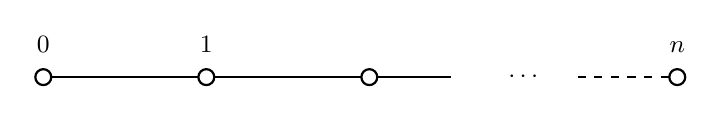
\begin{tikzpicture}[scale=1.15, >=stealth, every node/.style={font=\small}]

    % --- 1. x座標の基準定義 ---
    % xZero: 世代 0, xOne: 世代 1, xMid: 中間ノード, xDots: 省略部, xN: 世代 n
    \def\xZero{0.0}
    \def\xOne{1.8}
    \def\xMid{3.6}
    \def\xDots{5.3}
    \def\xN{7.0}
    \def\yLevel{0.0}

    % --- 2. 座標の定義 ---
    \coordinate (G0)   at (\xZero, \yLevel);
    \coordinate (G1)   at (\xOne,  \yLevel);
    \coordinate (GMid) at (\xMid,  \yLevel);
    \coordinate (GN)   at (\xN,    \yLevel);

    % --- 3. 枝（線分）の描画 ---
    % 世代 0 から世代 1、そして中間ノードへの進行
    \draw[thick] (G0) -- (G1) -- (GMid);

    % 中間ノードから省略ドット・点線を経て世代 n へ
    \draw[thick] (GMid) -- ++(0.9, 0);
    \node at (\xDots, \yLevel) {$\cdots$};
    \draw[thick, dashed] (\xDots + 0.6, \yLevel) -- (GN);

    % --- 4. ノード（白抜き円 ○）とラベル ---
    \draw[thick, fill=white] (G0)   circle (2.5pt) node[above=5pt] {$0$};
    \draw[thick, fill=white] (G1)   circle (2.5pt) node[above=5pt] {$1$};
    \draw[thick, fill=white] (GMid) circle (2.5pt);
    \draw[thick, fill=white] (GN)   circle (2.5pt) node[above=5pt] {$n$};

  \end{tikzpicture}
  \caption{世代 $0$ から世代 $n$ まで常に $1$ 個をキープするケース}
  \label{fig:generation_tree_single_line}
\end{figure}

第 $n$ 世代に $1$ 個あるのは，常に 1 個ずつの個体をのこす時で，確率は
\begin{align}
  P_n(1) = p^n \label{eq:1}
\end{align}
である．以下数式上の簡単さのため，$n=0$に対しても$P_n(1)=p^{0}=1$と定義する．

\paragraph{$P_n(2)$について}

\begin{figure}[htb]
  \centering
  \begin{tikzpicture}[scale=1.2, >=stealth, every node/.style={font=\small}]
    % --- 1. 座標の定義 ---
    \coordinate (O)  at (0, 0);       % 世代 0
    \coordinate (M1) at (2, 0);       % 世代 m-1
    \coordinate (M_up)   at (3.5, 0.85); % 世代 m (上)
    \coordinate (M_down) at (3.5, -0.85);% 世代 m (下)

    % 省略用の点々 (dots) の位置
    \coordinate (dot_up)   at (5.0, 0.85);
    \coordinate (dot_down) at (5.0, -0.85);

    % 世代 n の位置
    \coordinate (N_up)   at (6.5, 0.85); % 世代 n (上)
    \coordinate (N_down) at (6.5, -0.85);% 世代 n (下)

    % --- 2. 線の描画 ---
    % 実線部分
    \draw[thick] (O) -- (M1);
    \draw[thick] (M1) -- (M_up);
    \draw[thick] (M1) -- (M_down);
    \draw[thick] (M_up) -- (4.5, 0.85);
    \draw[thick] (M_down) -- (4.5, -0.85);

    % 省略部分 (ドット) と点線
    \node at (dot_up) {$\cdots$};
    \node at (dot_down) {$\cdots$};
    \draw[thick, dashed] (5.5, 0.85) -- (N_up);
    \draw[thick, dashed] (5.5, -0.85) -- (N_down);

    % --- 3. ノード（白抜き円 ○）とラベル ---
    \draw[thick, fill=white] (O) circle (2.5pt) node[left=4pt] {$0$};

    \draw[thick, fill=white] (M1) circle (2.5pt) node[above left=2pt] {$m-1$};

    \draw[thick, fill=white] (M_up) circle (2.5pt) node[above=4pt] {$m$};
    \draw[thick, fill=white] (M_down) circle (2.5pt) node[below=4pt] {$m$};

    \draw[thick, fill=white] (N_up) circle (2.5pt) node[above=4pt] {$n$};
    \draw[thick, fill=white] (N_down) circle (2.5pt) node[above=4pt] {$n$};

  \end{tikzpicture}
  \caption{世代 $0$ から世代 $m-1$，$m$ を経て世代 $n$ に至るケース}
  \label{fig:generation_tree}
\end{figure}

第 $n$ 世代に 2 個あるのは，第 $m$ 世代になった時に ($m=1, 2, \dots, n$) 1 個から 2 個になり，その後 $2$個の状態をキープした場合である．このような確率$q(m,n)$は
\begin{align}
  q(m,n) = P_{m-1}(1) \cdot (1-p) \{ p^{n-m} \}^2
\end{align}
である．ただし，$m=1$の時も(1)より$P_{0}(1)=1$でこの式は成り立つ．

従って，求める確率は$q(m,n)$を$m$について足し合わせて
\begin{align}
  P_n(2)
  &= \sum_{m=1}^n P_{m-1}(1) (1-p) p^{2n-2m} \\
  &= \sum_{m=1}^n p^{m-1} (1-p) p^{2n-2m} \quad (\because \text{\cref{eq:1}})\\
  &= (1-p) p^{2n-1} \sum_{m=1}^n \Bigl(\dfrac{1}{p}\Bigr)^m \\
  &= \dfrac{1}{p} \dfrac{1-(1/p)^n}{1-1/p} (1-p) p^{2n-1} \\
  &= (1-p^n) p^{n-1}\label{eq:2}
\end{align}
である．

\paragraph{$P_n(3)$について}

\begin{figure}[htb]
  \centering
  \begin{tikzpicture}[scale=1.15, >=stealth, every node/.style={font=\small}]

    % --- 1. x座標の基準定義 ---
    % x0: 手前, x_m1: 世代 m-1, x_m: 世代 m, x_dots: 省略部, x_n: 世代 n
    \def\xZero{0.0}
    \def\xMone{1.8}
    \def\xM{3.6}
    \def\xDots{5.3}
    \def\xN{7.0}

    % --- 2. y座標の基準定義 ---
    % 上の枝 (分裂後): yTop, 中央の枝 (分裂後): yMid, 下の枝 (そのまま): yBot
    \def\yTop{1.0}
    \def\yMid{0.0}
    \def\yBot{-1.1}
    \def\yBranchInit{0.5} % 分裂前の上の枝の高さ

    % --- 3. 座標の定義 ---
    % (a) 上側の系統（世代 m-1 から世代 m で2つに分裂）
    \coordinate (P_prev_top) at (\xZero, \yBranchInit);
    \coordinate (P_m1_top)   at (\xMone, \yBranchInit);
    \coordinate (P_m_top)    at (\xM, \yTop);
    \coordinate (P_m_mid)    at (\xM, \yMid);
    \coordinate (P_n_top)    at (\xN, \yTop);
    \coordinate (P_n_mid)    at (\xN, \yMid);

    % (b) 下側の系統（分裂せず進む）
    \coordinate (P_prev_bot) at (\xZero, \yBot);
    \coordinate (P_m1_bot)   at (\xMone, \yBot);
    \coordinate (P_m_bot)    at (\xM, \yBot);
    \coordinate (P_n_bot)    at (\xN, \yBot);

    % --- 4. 枝（線分）の描画 ---
    % 上側系統: 世代 m-1 までの直線と、世代 m への分岐
    \draw[thick] (P_prev_top) -- (P_m1_top);
    \draw[thick] (P_m1_top) -- (P_m_top);
    \draw[thick] (P_m1_top) -- (P_m_mid);

    % 上側系統: 世代 m から世代 n への進行（実線・省略ドット・点線）
    \draw[thick] (P_m_top) -- ++(1.0, 0);
    \node at (\xDots, \yTop) {$\cdots$};
    \draw[thick, dashed] (\xDots + 0.6, \yTop) -- (P_n_top);

    \draw[thick] (P_m_mid) -- ++(1.0, 0);
    \node at (\xDots, \yMid) {$\cdots$};
    \draw[thick, dashed] (\xDots + 0.6, \yMid) -- (P_n_mid);

    % 下側系統: 直線進行（実線・省略ドット・点線）
    \draw[thick] (P_prev_bot) -- (P_m1_bot) -- (P_m_bot) -- ++(1.0, 0);
    \node at (\xDots, \yBot) {$\cdots$};
    \draw[thick, dashed] (\xDots + 0.6, \yBot) -- (P_n_bot);

    % --- 5. ノード（白抜き円 ○）の描画 ---
    % 世代 m-1 の手前
    \draw[thick, fill=white] (P_prev_top) circle (2.5pt);
    \draw[thick, fill=white] (P_prev_bot) circle (2.5pt);

    % 世代 m-1
    \draw[thick, fill=white] (P_m1_top) circle (2.5pt) node[above=5pt] {$m-1$};
    \draw[thick, fill=white] (P_m1_bot) circle (2.5pt);

    % 世代 m
    \draw[thick, fill=white] (P_m_top) circle (2.5pt) node[above=5pt] {$m$};
    \draw[thick, fill=white] (P_m_mid) circle (2.5pt);
    \draw[thick, fill=white] (P_m_bot) circle (2.5pt);

    % 世代 m と省略ドットの間のノード（スケッチにある中間ノード）
    \draw[thick, fill=white] ($ (P_m_top) + (1.0, 0) $) circle (2.5pt);

    % 世代 n (合計3個)
    \draw[thick, fill=white] (P_n_top) circle (2.5pt) node[above=5pt] {$n$};
    \draw[thick, fill=white] (P_n_mid) circle (2.5pt);
    \draw[thick, fill=white] (P_n_bot) circle (2.5pt);

  \end{tikzpicture}
  \caption{世代 $m-1$ で $2$ 個のうち一方が世代 $m$ で分裂し，世代 $n$ で $3$ 個に至るケース}
  \label{fig:generation_tree_branch_3}
\end{figure}

さいごに第 $n$ 世代で 3 個となる時，第 $m$ 世代の時にはじめて 2 個から 3 個となるような $m$ ($m=2, 3, \dots, n$) がある．このような確率$r(m,n)$は
\begin{align}
  r(m,n)
  &= P_{m-1}(2) \cdot 2 \cdot p (1-p) \{ p^{n-m} \}^3 \\
  &= 2(1-p^{m-1}) p^{m-2} \cdot p(1-p) p^{3n-3m} \\
  &= 2(1-p) p^{3n-1} (1-p^{m-1}) p^{-2m} \\
  &= 2(1-p) p^{3n-1} (p^{-2m} - p^{-m-1})
\end{align}
である．ただし，$1$行目の係数$2$は2個の個体のうちどちらが$2$個に分裂するかで$2$通りある分の係数である．

より，$n \ge 2$ に対して，$P_n(3)$は$r(m,n)$を足し上げたもので
\begin{align}
  P_n(3)
  &= \sum_{m=2}^{n} r(m,n) \\
  &= 2(1-p) p^{3n-1} \sum_{m=2}^n \Bigl\{ \Bigl(\dfrac{1}{p^2}\Bigr)^m - \Bigl(\dfrac{1}{p}\Bigr)^{m+1} \Bigr\} \label{eq:3}
\end{align}
である．ここで
\begin{align}
  \begin{cases}
    \sum_{m=2}^n \Bigl(\dfrac{1}{p^2}\Bigr)^m = \dfrac{1}{p^4} \dfrac{1-(1/p^2)^{n-1}}{1-1/p^2} = \dfrac{1-(1/p^2)^{n-1}}{(p^2-1)p^2} \\
    \sum_{m=2}^n \Bigl(\dfrac{1}{p}\Bigr)^{m+1} = \dfrac{1}{p^3} \dfrac{1-(1/p)^{n-1}}{1-1/p} = \dfrac{1-(1/p)^{n-1}}{(p-1)p^2}
  \end{cases}
\end{align}
を\cref{eq:3}に代入して
\begin{align}
  P_n(3)
  &= 2(1-p) p^{3n-1} \Bigl[ \dfrac{1-(1/p^2)^{n-1}}{(p^2-1)p^2} - \dfrac{1-(1/p)^{n-1}}{(p-1)p^2} \Bigr] \\
  &= 2 p^{3n-3} \Bigl[ 1 - (1/p)^{n-1} - \dfrac{1-(1/p^2)^{n-1}}{1+p} \Bigr] \\
  &= 2 \Bigl[ p^{3n-3} - p^{2n-2} - \dfrac{p^{3n-3}-p^{n-1}}{1+p} \Bigr] \\
  &= \dfrac{2}{1+p} \Bigl[ p^{3n-2} - (1+p) p^{2n-2} + p^{n-1} \Bigr] \label{eq:4}
\end{align}
である．
$n=1$ の時は$P_1(3)=0$ で\cref{eq:4}の表示で良い．
よって
\begin{align}
  P_n(3) = \dfrac{2}{1+p} \Bigl[ p^{3n-2} - (1+p) p^{2n-2} + p^{n-1} \Bigr]
\end{align}
である．

\end{document}
